\documentclass[b5paper,10pt,twoside,openright]{memoir}
%%%%%%%%%%%%%%%%%%%%%%%%%%%%%%%%%%%%
% Load preamble from separate file %
%%%%%%%%%%%%%%%%%%%%%%%%%%%%%%%%%%%%
\usepackage{./style/MyPhDThesis}
%%%%%%%%%%%%%%%%%%%%%%%%%%%%%%%
% Author and document details %
%%%%%%%%%%%%%%%%%%%%%%%%%%%%%%%
\title{Ductile Fracture of Aluminium Sheet Under Combined \\ Tension-Compression Loading}
\author{Astrid Solheim}
\city{Trondheim}
\country{Norway}
\date{\today}
\faculty{Engineering}
\department{Structural Engineering}
\ISBNprinted{978-82-000-0000-0}
\ISBNelectronic{978-82-000-0000-1}
\serialNumber{\the\year :12}
%%%%%%%%%%%%%%%%%%%%%%%%%
% Begin PhD Thesis here %
%%%%%%%%%%%%%%%%%%%%%%%%%
\begin{document}
%%%%%%%%%%%%%%%%%%%%
%%%  Title page  %%%
%%%%%%%%%%%%%%%%%%%%
\frontmatter
\maketitle
%%%%%%%%%%%%%%%%%%%%%%%%%%%%%%%%%%%%%%%%%%
% Preface, abstract, and acknowledgement %
%%%%%%%%%%%%%%%%%%%%%%%%%%%%%%%%%%%%%%%%%%
\pagestyle{plain}
\pagenumbering{roman}
%%%%%%%%%%%
% Preface %
%%%%%%%%%%%
\chapter*{Preface}

This thesis is submitted in partial fulfilment of the requirements for the
degree of Philosophiae Doctor at the Norwegian University of Science and
Technology (NTNU). The work was carried out at the Department of Structural
Engineering between 2022 and 2026, under the supervision of a project
studying the low-triaxiality fracture behaviour of aluminium alloys used in
automotive crash structures.

The thesis is article-based: the main synopsis chapters summarise the
motivation, methodology and conclusions of the work as a whole, and the two
papers reproduced in full afterwards carry the detailed derivations, test
data and validation results.

\vspace{\fill}
\prefaceSignature

\addcontentsline{toc}{chapter}{Preface}
\cleardoublepage
%%%%%%%%%%%%
% Abstract %
%%%%%%%%%%%%
\chapter*{Abstract}

Automotive crash structures rely on aluminium components that see stress
states ranging from uniaxial tension to combined compression-shear during a
single impact event, yet most fracture-model calibration campaigns are built
almost entirely from tension-dominated specimens. This thesis addresses that
gap for cold-rolled AA6082 sheet, combining a rate-dependent necking study
with a damage-coupled fracture model calibrated jointly across tension- and
compression-dominated stress states.

Paper 1 characterises the rate dependence of diffuse necking onset in
AA6082-T6 sheet across four decades of strain rate, and shows that a modified
Considère criterion with a single rate-sensitivity parameter predicts the
observed onset strains to within 6\%. Paper 2 extends a local damage-coupled
constitutive model into the low- and negative-triaxiality regime using a
purpose-built compression-shear specimen, and shows that models calibrated
on tension data alone systematically over-predict ductility in this regime.

Together, the two papers give a calibration and validation route for
predicting ductile fracture in aluminium sheet across the full range of
stress states relevant to a crash event, rather than the tension-dominated
subset typically covered.

\addcontentsline{toc}{chapter}{Abstract}
\cleardoublepage
%%%%%%%%%%%%%%%%%%%%
% Acknowledgements %
%%%%%%%%%%%%%%%%%%%%
\chapter*{Acknowledgements}

I would like to thank my supervisors for their guidance throughout this
project, the structures laboratory technical staff for their help with the
compression-shear fixture design, and my fellow PhD candidates in the
research group for many useful discussions.

\addcontentsline{toc}{chapter}{Acknowledgements}
\cleardoublepage
%%%%%%%%%%%%%%%%%%%%%
% Table of contents %
%%%%%%%%%%%%%%%%%%%%%
\tableofcontents*
\cleardoublepage
%%%%%%%%%%%%%%%%%%%%%%%%
%%%% Main document %%%%%
%%%%%%%%%%%%%%%%%%%%%%%%
\mainmatter
%%%%%%%%%%%%%%%%%%%
%%%% Synopsis %%%%%
%%%%%%%%%%%%%%%%%%%
\begingroup % Remove new page after new chapter after Synopsis
\renewcommand{\cleardoublepage}{}
\renewcommand{\clearpage}{}
\titlespacing*{\chapter}{0pt}{0pt}{0pt} % Sets spacing to zero between Synopsis and Introduction
\chapter*{{\Huge Synopsis}}
\label{Ch:synopsis}
\addcontentsline{toc}{part}{Synopsis}
%%%%%%%%%%%%%
%% Content %%
%%%%%%%%%%%%%
\titlespacing*{\chapter}{0pt}{0pt}{25pt}
\chapter{Introduction}
\label{Ch:Introduction}

Ductile fracture of aluminium alloys is a stress-state-dependent
phenomenon: the strain to failure of a given alloy varies by more than a
factor of two between uniaxial tension and shear-dominated loading
\citep{Bao.2004}. Automotive crash structures routinely see both regimes
within a single impact pulse, so a fracture model calibrated only on
tension-dominated specimens can substantially over-predict the ductility
available in the compression-shear regions of a deforming component
\citep{Bai.2010}.

This thesis addresses that gap for cold-rolled AA6082 sheet, an alloy
commonly used in extruded and sheet automotive crash components. The work
combines a rate-dependent characterisation of necking onset with a
damage-coupled fracture model extended into the low- and
negative-triaxiality regime, calibrated jointly across a tension- and a
compression-dominated specimen set.

\endgroup
\chapter{Objectives and scope}
\label{Ch:ObjectivesScope}

\section{Objectives}
\label{Sec:Objectives}

The objectives of this thesis are to:

\begin{enumerate}
    \item Characterise the rate dependence of diffuse necking onset in
    cold-rolled AA6082-T6 sheet across a wide range of strain rates.
    \item Extend a local damage-coupled fracture model into the low- and
    negative-triaxiality stress-state regime using a dedicated
    compression-shear specimen.
    \item Evaluate whether a fracture model calibrated jointly across
    tension- and compression-dominated specimens improves fracture
    predictions relative to one calibrated on tension data alone.
\end{enumerate}

\section{Scope}
\label{Sec:Scope}

The experimental and modelling work in this thesis is restricted to
AA6082-T6 sheet at room temperature and quasi-static to moderate strain
rates ($10^{-3}$--$10^{2}$~s$^{-1}$). Temperature effects, cyclic loading,
and alloys other than AA6082 are outside the scope of this thesis, though
the compression-shear specimen design and calibration methodology developed
here are not alloy-specific.

\chapter{Research methodology}
\label{Ch:Methodology}

The work in this thesis follows an experiment-then-model approach common in
structural impact research. Paper 1 is purely experimental: uniaxial tensile
tests at four strain rates, instrumented with digital image correlation, to
characterise necking onset. Paper 2 is a combined experimental-modelling
study: a new compression-shear specimen geometry was designed and tested
alongside conventional notched-bar tension specimens, and the resulting data
were used to calibrate and validate a damage-coupled constitutive model
against an independent, fourth geometry not used in calibration.

All mechanical testing was performed on the same servo-hydraulic test rig at
the Structural Impact Laboratory, using the same digital image correlation
setup for strain-field measurement, so that the necking-onset criterion from
Paper 1 and the damage model from Paper 2 are calibrated against consistent
strain measurements throughout.

\chapter{Summary}
\label{Ch:Summary}

\section{Part 1}
\begin{itemize}
    \item[{[1]}] Solheim, A., Vartdal, K., Aune, M. (2025). \textit{Rate-dependent necking onset in cold-rolled AA6082 sheet.} International Journal of Fracture (submitted).
\end{itemize}

\section{Part 2}
\begin{itemize}
    \item[{[2]}] Solheim, A., Vartdal, K. (2026). \textit{A local damage-coupled model for ductile fracture under combined tension-compression loading.} International Journal of Plasticity (submitted).
\end{itemize}

\chapter{Concluding remarks and further work}
\label{Ch:ConcludingRemarksFurtherWork}

The two papers in this thesis together give a calibration and validation
route for ductile-fracture prediction in aluminium sheet across the full
range of stress states seen in a crash event, rather than the
tension-dominated subset typically covered. The rate-dependent necking
criterion from Paper 1 and the triaxiality-dependent damage model from
Paper 2 share a common experimental basis, which is what allows the two to
be combined directly in a crash simulation without a separate
re-calibration step.

Further work should extend the compression-shear specimen and calibration
methodology to other automotive aluminium alloys, and evaluate whether the
rate-sensitivity parameter identified in Paper~1 needs to be re-calibrated
at the higher strain rates seen in a real crash pulse, which exceed the
$10^{2}$~s$^{-1}$ upper bound tested here.

\cleardoublepage
%%%%%%%%%%%%%%%%
%% References %%
%%%%%%%%%%%%%%%%
\printbibliography[title=References, heading=bibliography]
\cleardoublepage
%%%%%%%%%%%%%%%%%%%
%%%% Articles %%%%%
%%%%%%%%%%%%%%%%%%%
\addcontentsline{toc}{part}{Articles}
%%%%%%%%%%%%%%%
%% Part page %%
%%%%%%%%%%%%%%%
\tocless\part{}\label{Part1}
\parttext{
\begin{flushleft}
\vspace{-.10\textheight}
\begin{minipage}{\linewidth}

A. Solheim, K. Vartdal, M. Aune

\vspace{1cm}

{\Large \textbf{Rate-dependent necking onset in cold-rolled AA6082 sheet}}

\vspace{0.5cm}

International Journal of Fracture (submitted).

\end{minipage}
\end{flushleft}
\vfill
}

\addcontentsline{toc}{section}{Rate-dependent necking onset in cold-rolled AA6082 sheet}
\cleardoublepage
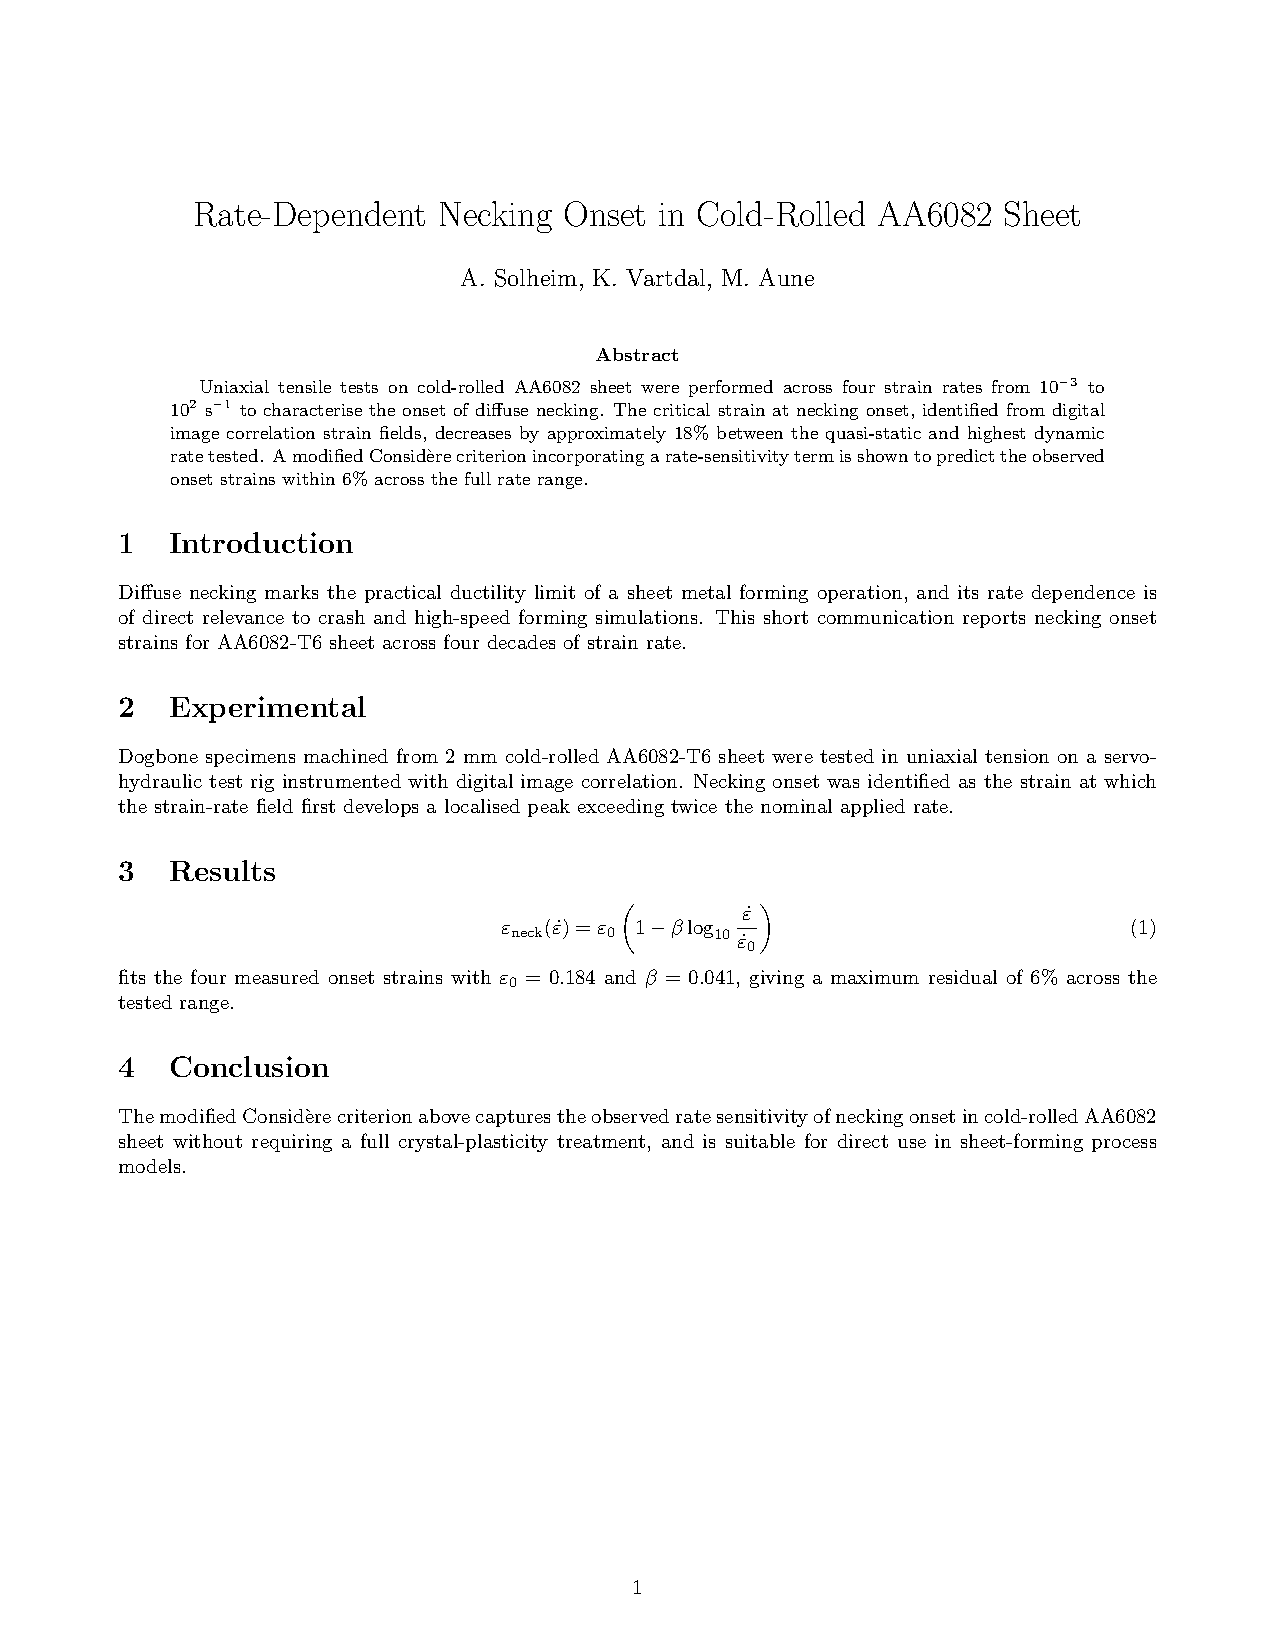
\includepdf[pages=-]{./articles/Paper1.pdf}
\cleardoublepage
%%%%%%%%%%%%%%%
%% Part page %%
%%%%%%%%%%%%%%%
\tocless\part{}\label{Part2}
\parttext{
\begin{flushleft}
\vspace{-.10\textheight}
\begin{minipage}{\linewidth}

A. Solheim, K. Vartdal

\vspace{1cm}

{\Large \textbf{A local damage-coupled model for ductile fracture under \\
combined tension-compression loading}}

\vspace{0.5cm}

International Journal of Plasticity (submitted).

\end{minipage}
\end{flushleft}
\vfill
}

\addcontentsline{toc}{section}{A local damage-coupled model for ductile fracture under combined tension-compression loading}
\cleardoublepage
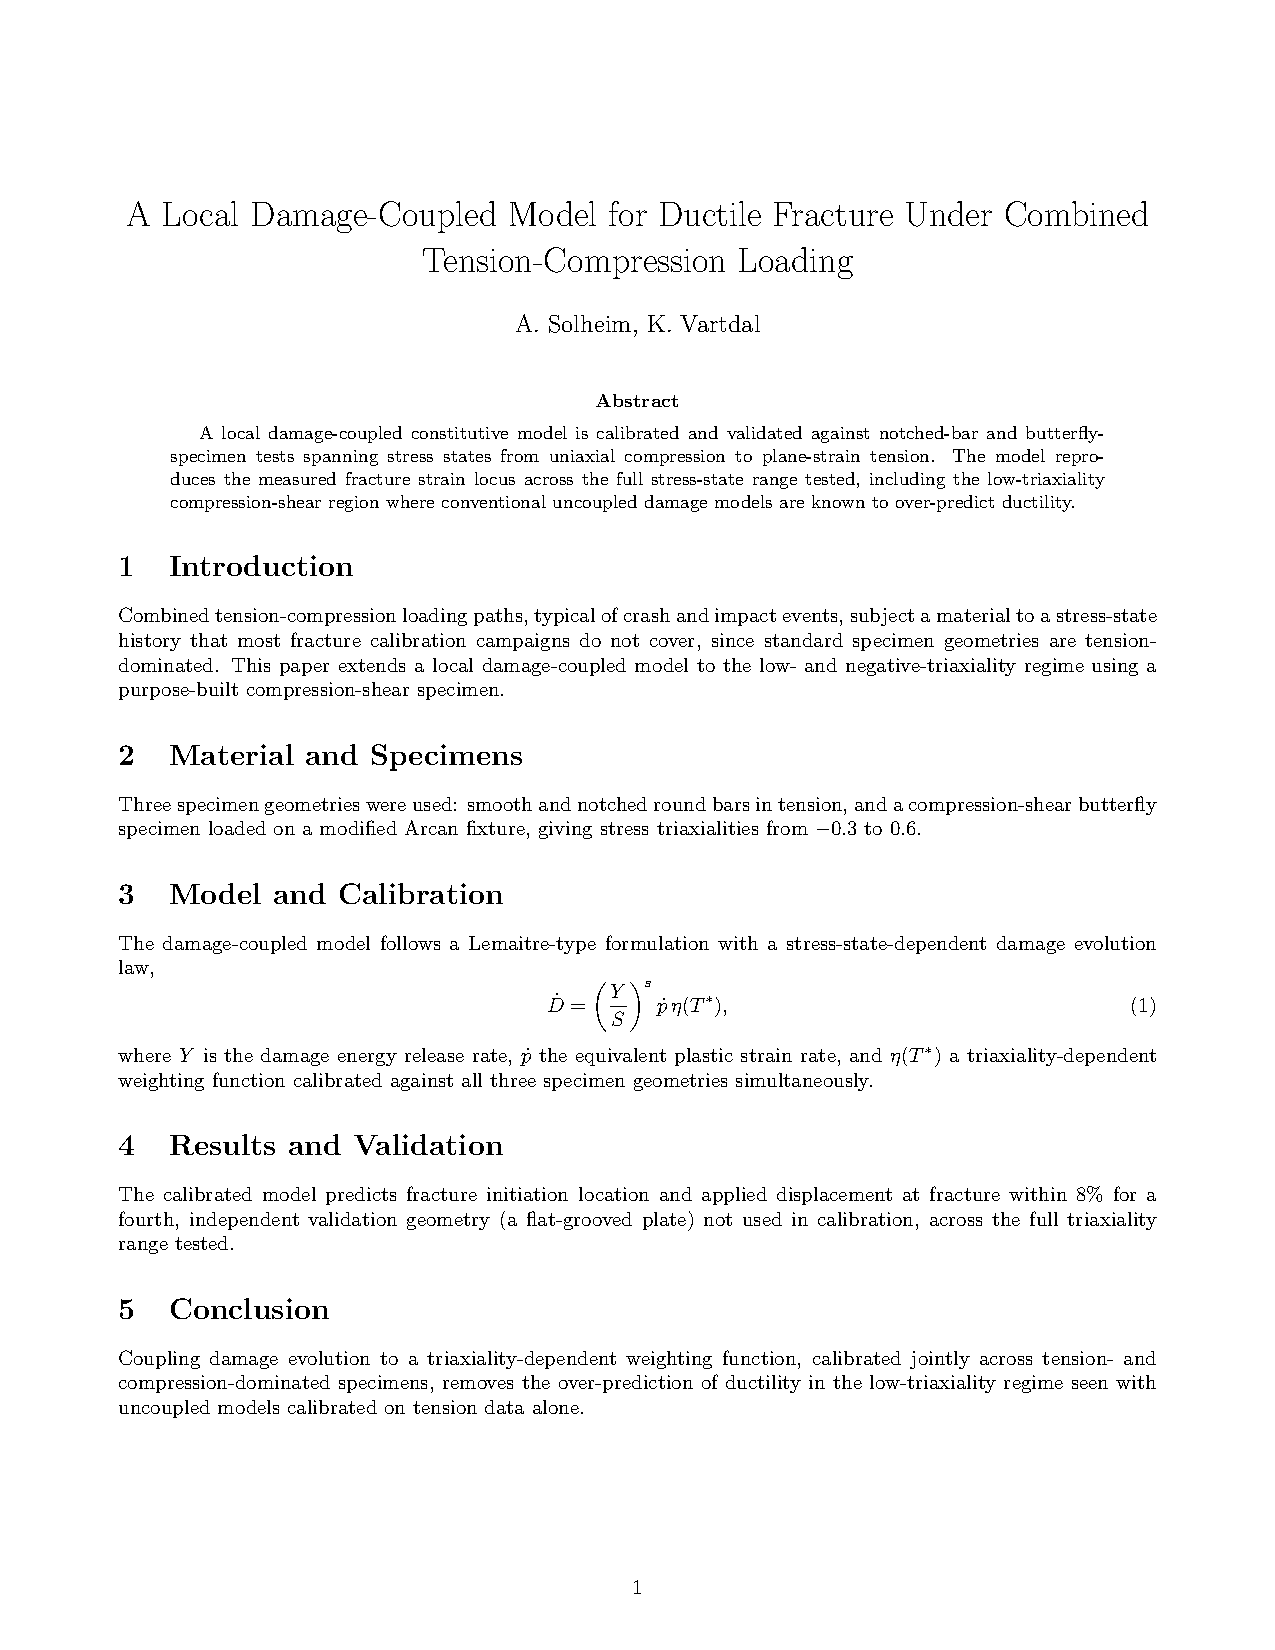
\includepdf[pages=-]{./articles/Paper2.pdf}
\cleardoublepage
%%%%%%%%%%%%%%%%%%%
%%%% Appendix %%%%%
%%%%%%%%%%%%%%%%%%%
\appendix
\appendixpage
\chapter{Compression-shear specimen drawings}
\label{Appendix:Appendix1}

This appendix would normally reproduce the full engineering drawings for the
compression-shear butterfly specimen used in Paper 2, including tolerances
and the modified Arcan fixture geometry. They are omitted from this starter
template; a real thesis appendix would include them as PDF or vector figures
alongside a brief note on machining tolerances achieved.

\cleardoublepage
%%%%%%%%%%%%%%%%
\end{document}
